% !TEX root = ../../sethomas_thesis_main.tex
\documentclass[border=1mm,
               class=article
               preview]{standalone}
% \usepackage{tikz}
% trim={<left> <lower> <right> <upper>}

\begin{document}
\begin{tikzpicture}
    \node[anchor=south west,inner sep=0] (graph) at (0,0) {
        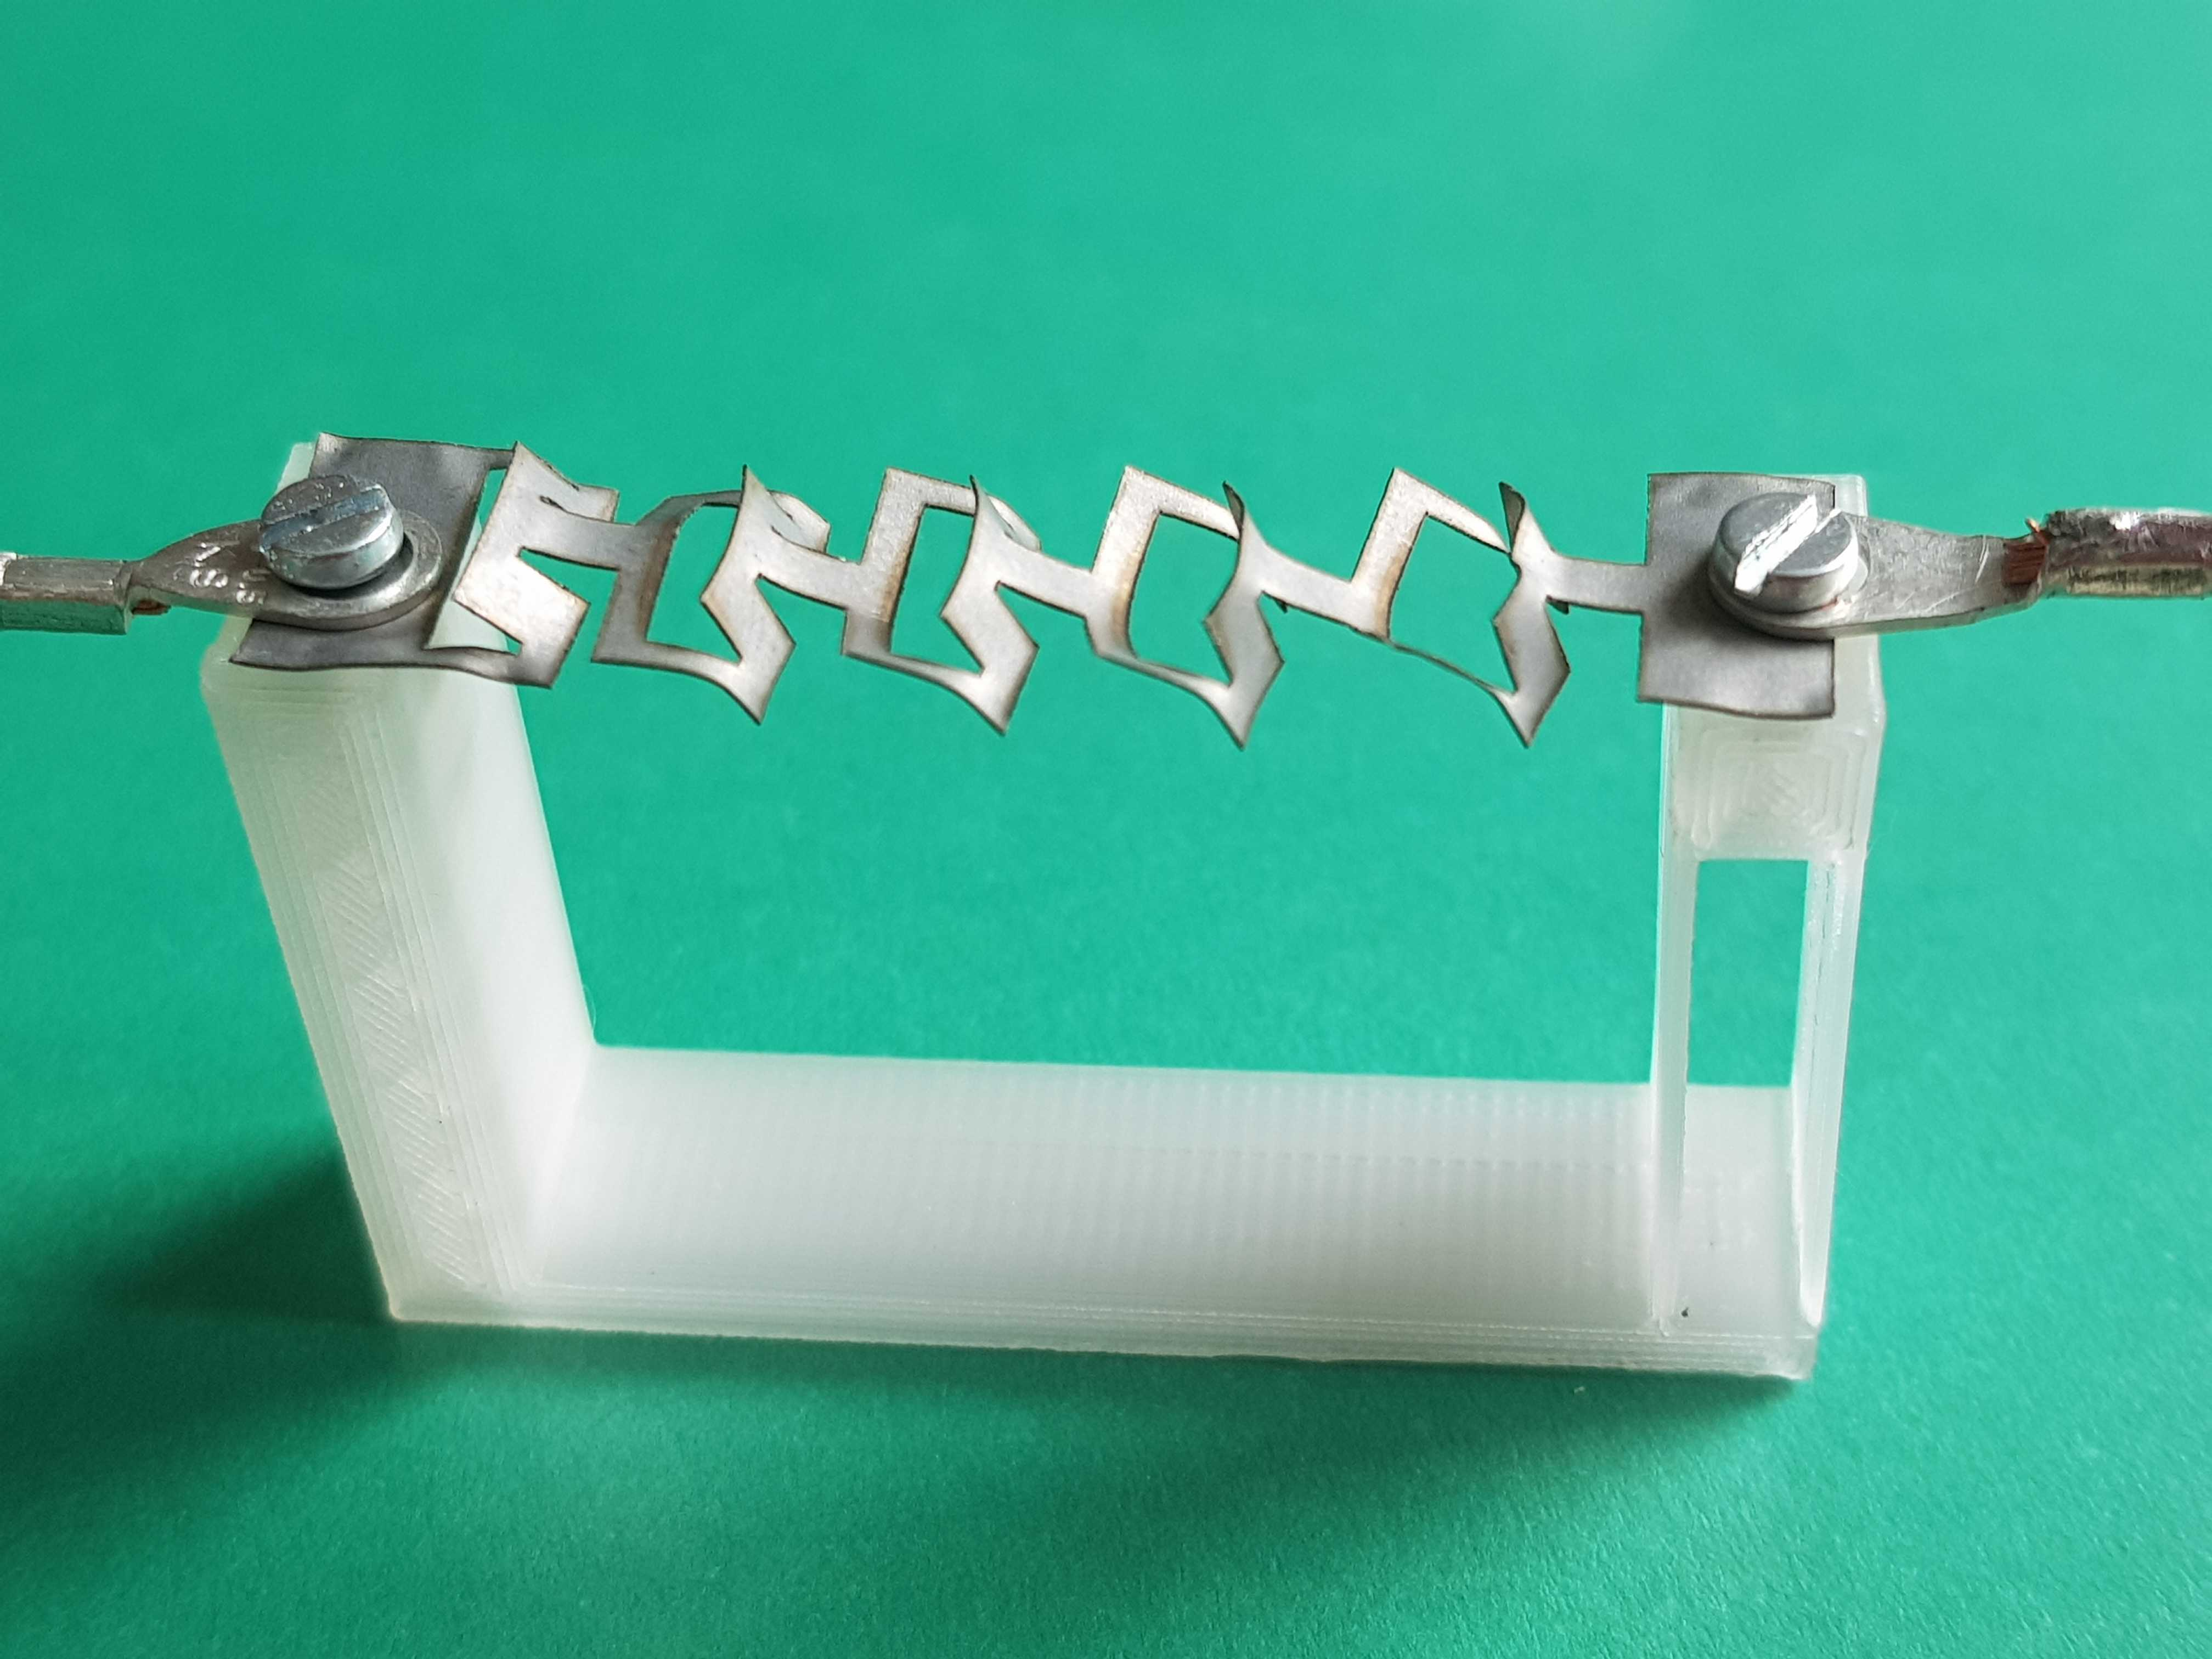
\includegraphics[trim={0 10cm 0 20cm}, clip]{images/chap5/sma-kiri-actuator-green-iso.jpg}
    };
    \begin{scope}[x={(graph.south east)},y={(graph.north west)}]
        \node[anchor=north west,inner sep=0] (graphsmall) at (0,-0.01) {
            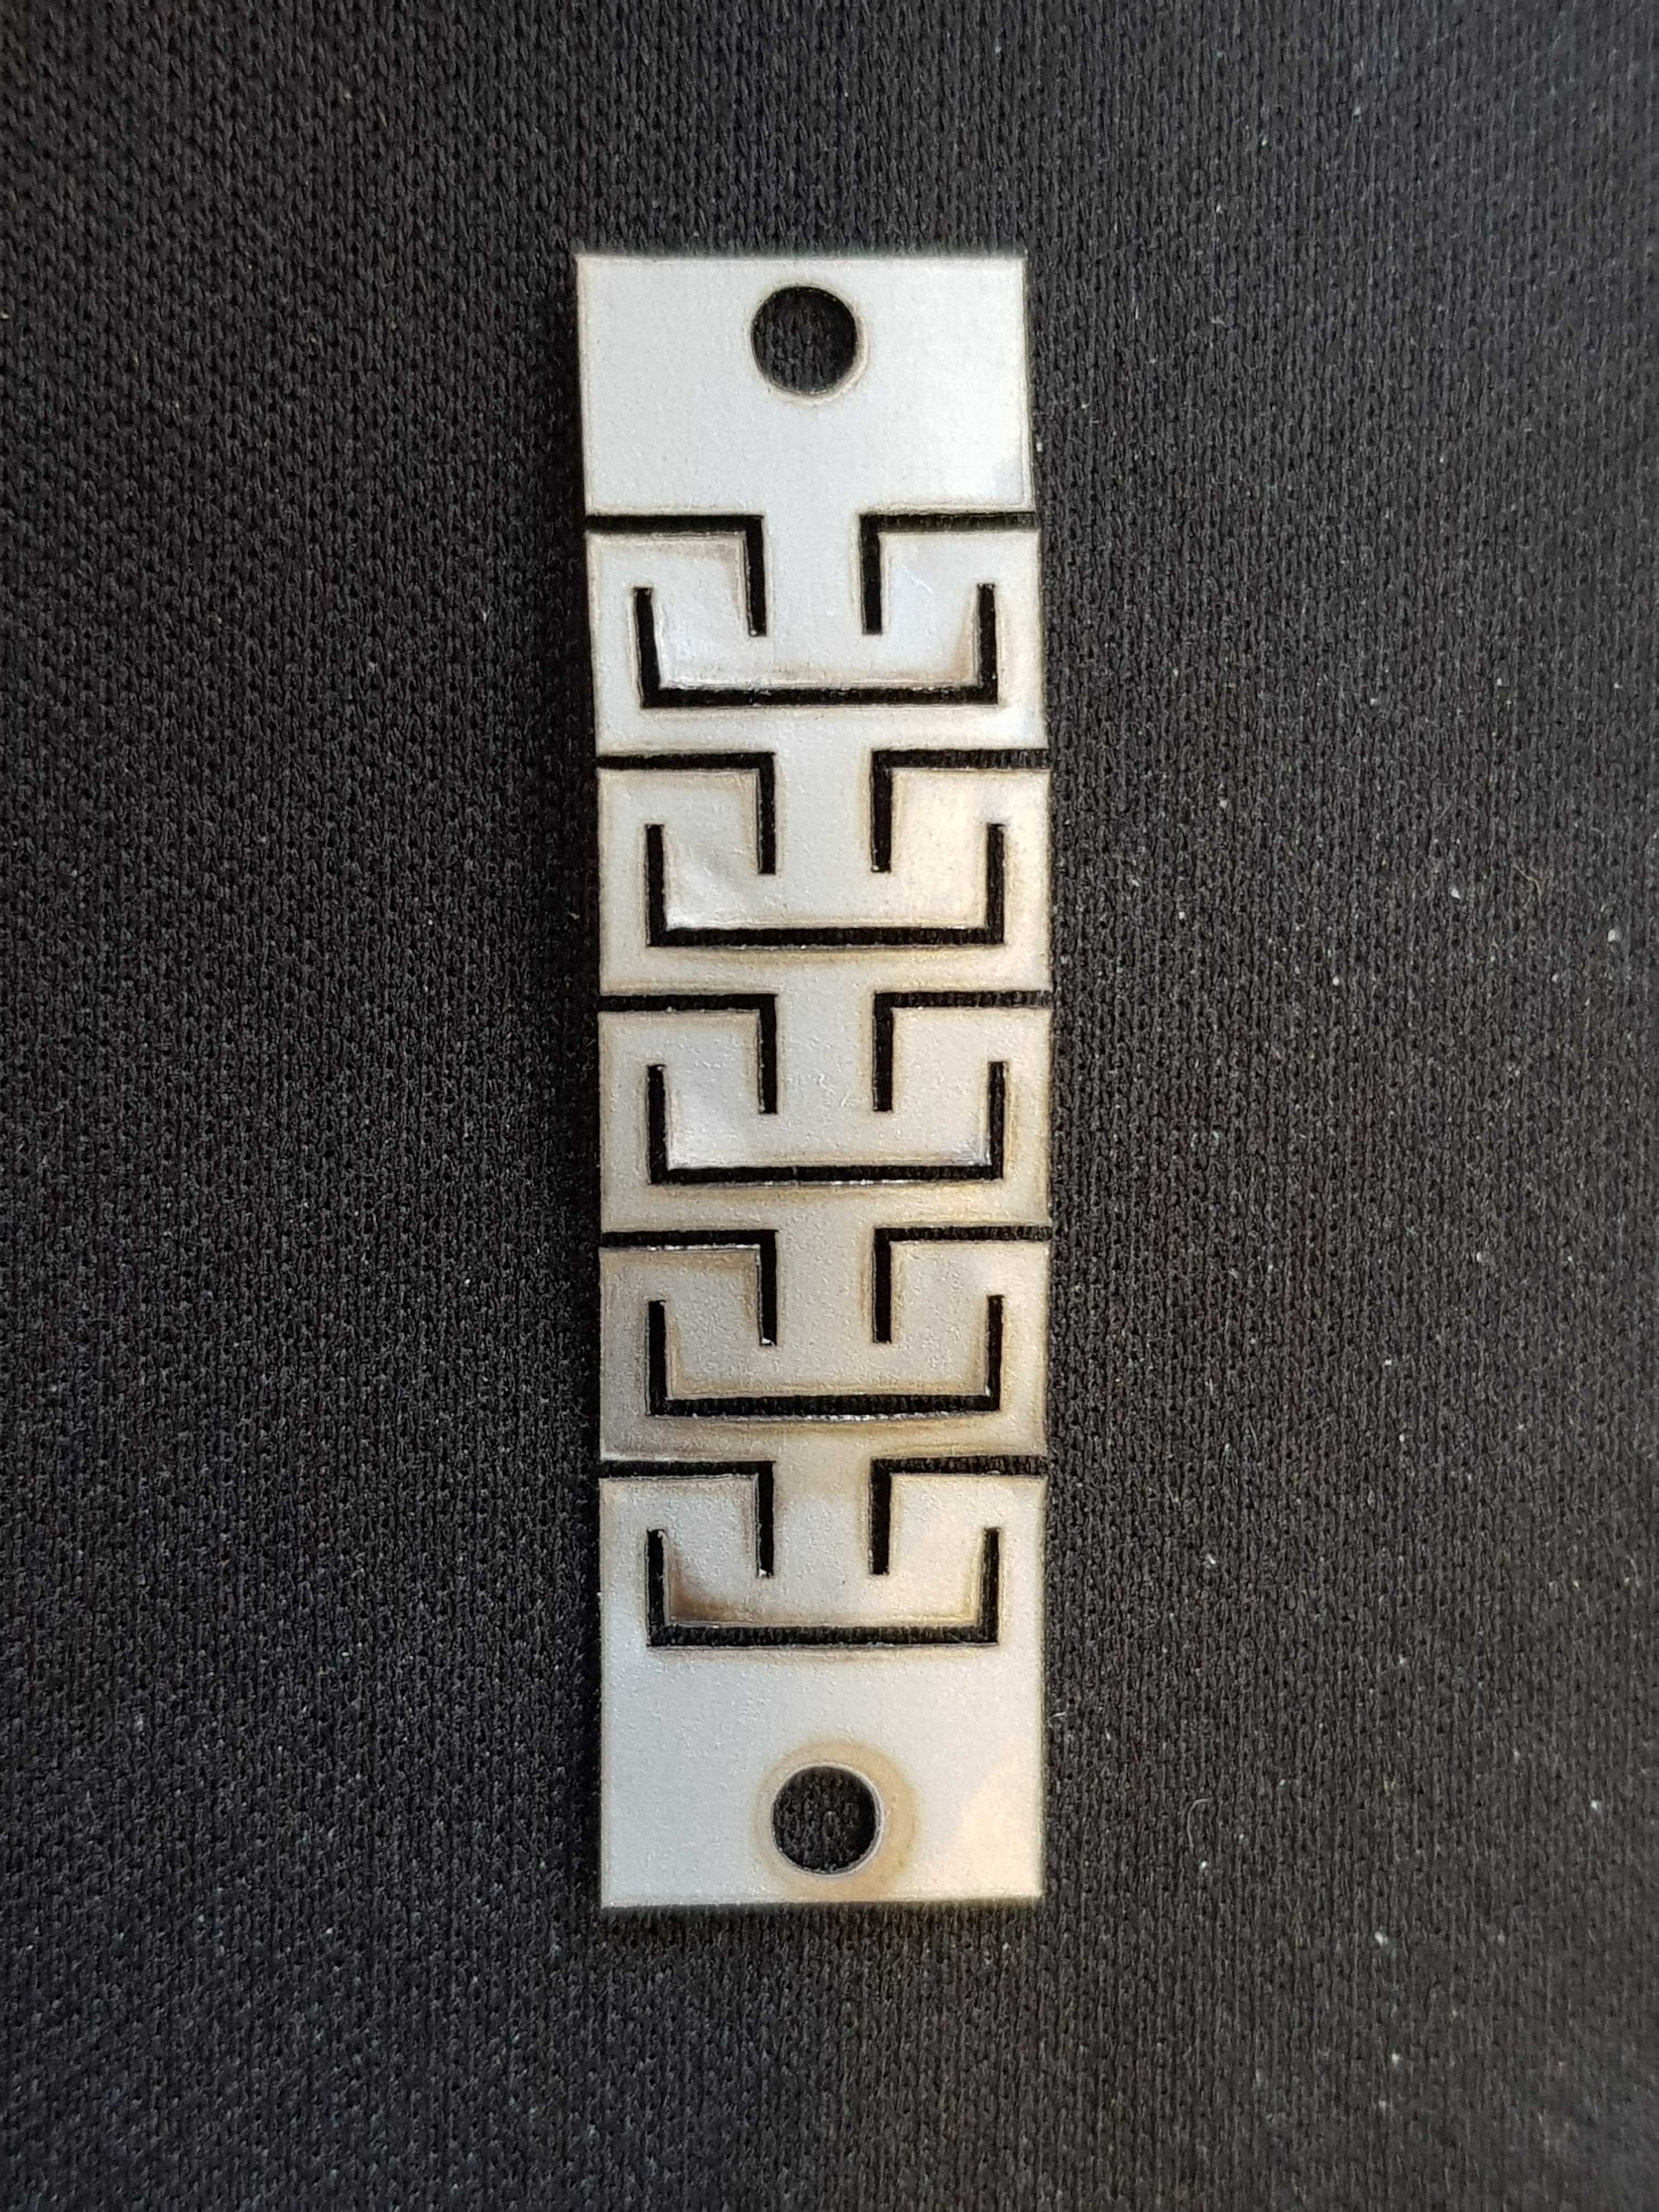
\includegraphics[trim={30cm 10cm 30cm 10cm}, clip, angle=90, scale=1.165]{images/chap5/sma-kiri-flat.jpg}
        };
        % \node[anchor=south west,inner sep=0] (graphsmall) at (0.02,0.02) {
        %     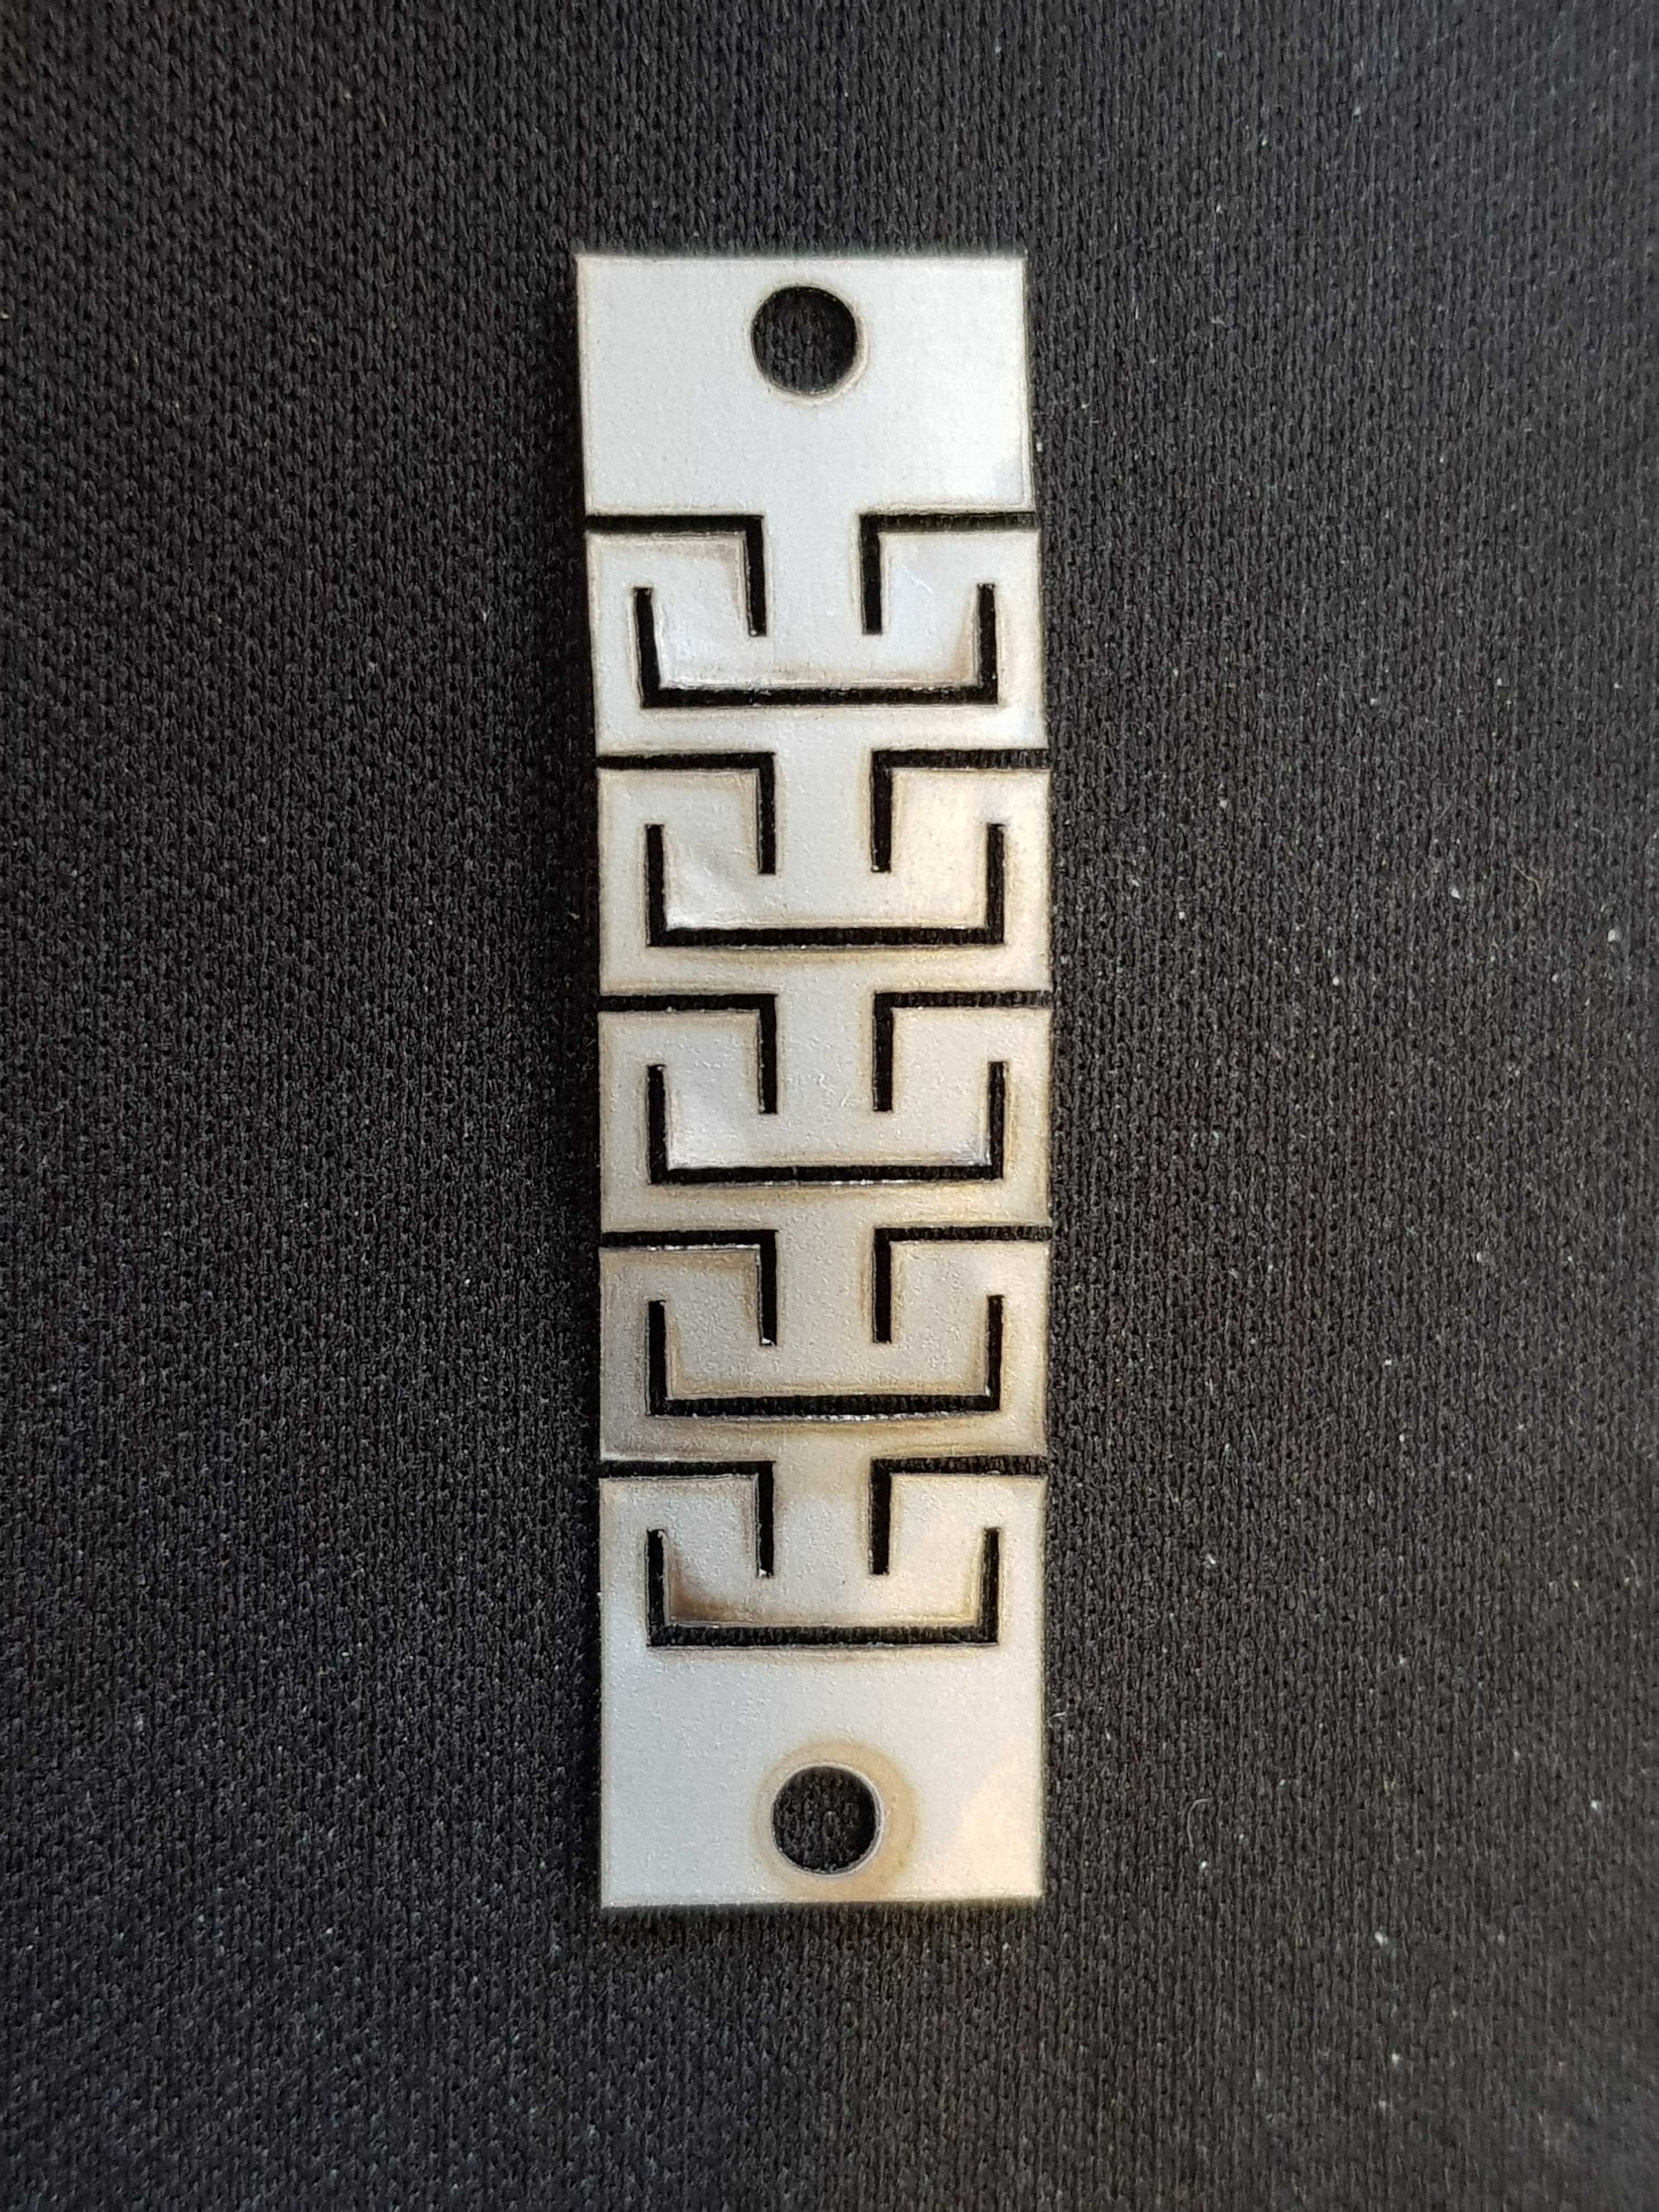
\includegraphics[trim={30cm 10cm 30cm 10cm}, clip, angle=90, scale=0.45]{images/chap5/sma-kiri-flat.jpg}
        % };
        \draw[white, line width=50pt] (0.82,0.05) -- (0.97,0.05);
        \node[white,scale=7.5,anchor=center] (scale) at (0.895,0.1){\huge 15 mm};
      % \draw[help lines,xstep=.05,ystep=.05] (0,0) grid (1,1);
      %   \foreach \x in {0,1,...,9} { \node [anchor=north] at (\x/10,0) {0.\x}; }
      %   \foreach \y in {0,1,...,9} { \node [anchor=east] at (0,\y/10) {0.\y}; }
    \end{scope}
    % \draw[lightcolor, ultra thick] (graph1x1.south east) rectangle (graph1x1.north west);
    % \draw[middlecolor, ultra thick] (graph2x1.south east) rectangle (graph2x1.north west);
    % \draw[darkcolor, ultra thick] (graph1x2.south east) rectangle (graph1x2.north west);



\end{tikzpicture}
\end{document}
